\section{Theory}
\subsection{Background knowledge}
The paper “Experimental Quantum Generative Adversarial Networks for Image Generation” proposes a new method for the task of image generation, which trains generative adversarial networks using the quantum computer. Generative Adversarial Networks (GANs) consist of two neural networks, a generator, and a discriminator. The job of the generator is to create synthetic data that is as close as possible to the real data, such as a text word or an image, whereas the discriminator tries to distinguish between the real data and generator-generated synthetic data. 

\subsection{Why we expect GANs to converge}
The training process of these two components can be traded as a min-max game. Formally, the objective function of a GANs can be expressed as a min-max function, where the generator tries to minimize the value of the function and the discriminator tries to maximize the function. The goal of the generator is to generate synthetic data in such a way that the difference between the distribution of the synthetic data and the distribution of the real data is minimized. The discriminator's goal is to correctly classify the data as real or synthetic by maximizing the difference between the distribution of the real data and the distribution of the synthetic data. We expected GANs to converge where the min-max game between the generator and the discriminator continues until the generator can no longer improve, or the discriminator can no longer distinguish between real and synthetic data. At this point, both two players have optimal strategies, GANs have achieved the goal of generating synthetic data that is indistinguishable from real data. 

\subsection{How to compute loss?}
Since the generator and discriminator have different objectives, the loss function is also different. It looks like this:
\[\min\limits_{\theta} \max\limits_{\gamma} \mathcal{L}\{D_{\gamma}{[G_{\theta}(z)], D_{\gamma}(x)}\} := \mathbb{E}_{x \sim P_{data}(x)}[\log D_{\gamma}(x)] + \mathbb{E}_{z \sim P(z)}(\log\{1 - D_{\gamma}[G_{\theta}(z)]\})\]
where $D_{\gamma}(x)$ is the discriminator's estimate of the probability that real data instance $x$ is real, $\mathbb{E}_{x \sim P_{data}(x)}$ is the expected value over all real data instances. $G_{\theta}(z)$ is the generator's output when given noise $z$. $D_{\gamma}[G_{\theta}(z)]$is the discriminator's estimate of the probability that a fake instance is real, and $\mathbb{E}_{z \sim P(z)}$ is the expected value over all random inputs to the generator. 

Specifically, for the discriminator, the loss is computed as the sum of the binary cross-entropy between the true labels (1 for real data and 0 for fake data) and the predicted probabilities. In other words, the discriminator aims to minimize the loss when correctly classifying real and fake examples. The lower the loss of the discriminator, the more effective the discriminator is in distinguishing between real and fake data.
For the generator, the loss is computed as the binary cross-entropy between the true labels and the discriminator's prediction of the generated data. The generator aims to maximize this loss because it means that the discriminator is classifying the synthetic examples as real. In other words, the generator aims to produce synthetic examples that minimize the discriminator's ability to distinguish between real and fake examples.

\subsection{How to compute gradients?}
Below is the process of how gradients are computed for a real vs fake example.
\begin{figure}[H]
    \centering
    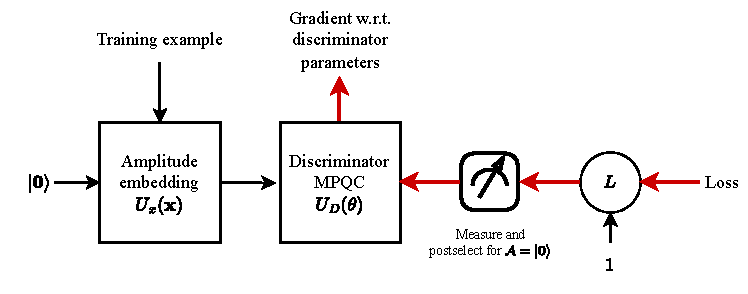
\includegraphics[width=0.7\textwidth]{figures/discrim_real.pdf}
    \caption{Gradients computation for the real example w.r.t. discriminator parameters.}
    \label{fig:bar_data}
\end{figure}

\begin{figure}[H]
    \centering
    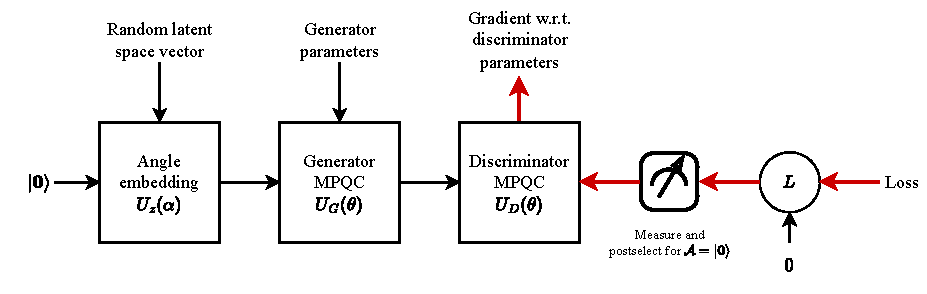
\includegraphics[width=0.8\textwidth]{figures/discrim_fake.pdf}
    \caption{Gradients computation for the fake example w.r.t. discriminator parameters.}
    \label{fig:bar_data}
\end{figure}

\begin{figure}[H]
    \centering
    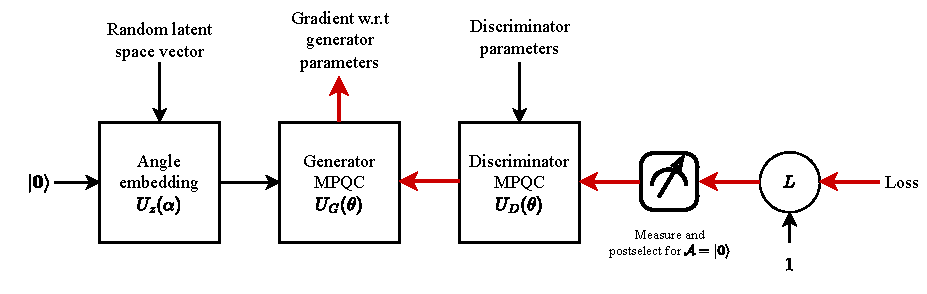
\includegraphics[width=0.8\textwidth]{figures/gen_fake.pdf}
    \caption{Gradients computation w.r.t. generator parameters.}
    \label{fig:bar_data}
\end{figure}


\subsection{Why does quantum GANs perform better than classical GANs?}
The paper mainly argues how quantum-implement GANs is more effective than classical GANs. We have concluded some points: 

First, because of the nature of quantum computers, it is able to complete image generation with high-dimensional features by exploiting quantum GANs to get $2^n$ size feature vectors with only $n$ qubits and could harness quantum superposition to train multiple examples in parallel, which could potentially speed up the training process. Second, by utilizing the randomness in the quantum circuit, we could possibly get more robust trained networks, thus getting improved performance on noisy data and better generalization. 

% TODO
% \subsection{How does non-linearity work?}
% In this section, we would like to show how a two-qubit system can implement a specific nonlinear function with post-selection.


